% Performance and Scaling of ug4 introduction {{{
The current project was part of the transition period from Comet to Expanse. We therefore present performance data for both architectures. 
\subsection*{General scaling properties of uG4}
Our base code \ug is parallelized using MPI and written in C++ and has been extensively benchmarked (Vogel et al., 2013; Heppner et al., 2013) and shown to scale beyond 200,000 processes. In order to test the code on the SDSC Comet supercomputer, we ran a test problem using the Laplace equation on a three-dimensional unit cube. The second order elliptic partial differential equation reads
\begin{equation}
\Delta \Phi = 0,
\end{equation}
where $\Phi$ is a scalar function in the domain $\Omega \subset \mathbf{R}^n$, and $\Delta$ is the Laplace operator.
Strong scaling is demonstrated for a domain consisting of 16,974,593 degrees of freedom, see Tab.~\ref{tab:xsede_strong_scaling} and Fig.~\ref{fig:speedup_laplace}. The execution time roughly halves when doubling the number of processes. A weak scaling study, see Tab.~\ref{tab:xsede_weak_scaling} and Fig.~\ref{fig:scaled_speedup_laplace} on SDSC Comet. With each refinement of the grid the degrees of freedom (DoFs) increase by a factor of 8 and thus we increased the number of processes eightfold in each refinement step.
% }}}

% {{{ 3d Laplace problem
\begin{center}
\begin{table}[H]
\centering
\begin{tabular}{lrrr} 
\toprule
\textbf{Strong scaling in \ug} \\
\midrule
\emph{DoFs} & \emph{Runtime [s]} & \emph{\# Processes} & \emph{\# Nodes}\\
\midrule 
16,974,593 & 41 &  24 & 1 \\
16,974,593 & 20 &  48 & 2 \\
16,974,593 & 14 &  72 & 3 \\
16,974,593 & 10 &  96 & 4 \\
16,974,593 &  8 & 120 & 5 \\
16,974,593 &  7 & 144 & 6 \\
16,974,593 &  5 & 168 & 7 \\
16,974,593 &  2 & 192 & 8 \\
\bottomrule
\end{tabular}
\caption{Runtimes of simulations of a \textit{3d Laplace problem} on a fixed unit
 cube domain (seven regular refinements) with uG4 on the SDSC Comet HPC cluster.
Note that each node can allocate at maximum 24 processes and the maximum number
of processes or cores per job is limited to 1,728 processes in total.}
\label{tab:xsede_strong_scaling}
\end{table}
\end{center}

\begin{center}
\begin{table}[H]
\centering
\begin{tabular}{lrrrr}
\toprule
\textbf{Weak scaling in \ug} \\
\midrule
\emph{DoFs} & \emph{Runtime [s]} & \emph{\# Processes} & \emph{\# Refinements} \\
\midrule 
27 & 5.06 & 1 & 0 \\
216 & 5.06 & 8 & 1 \\
1,726 & 6.92 & 64 & 2 \\
13,824 & 6.92 & 512 & 3 \\
110,592 & 5.50 & 4096 & 4 \\
\bottomrule
\end{tabular}
\caption{Runtimes of simulations of a \textit{3d Laplace problem} on a unit cube 
domain (different number of regular refinements) with \ug on the SDSC Comet HPC cluster.
Note that each grid refinement increases the DoFs by a factor 8.}
\label{tab:xsede_weak_scaling}
\end{table}
\end{center}


\begin{figure}[H]
\centering
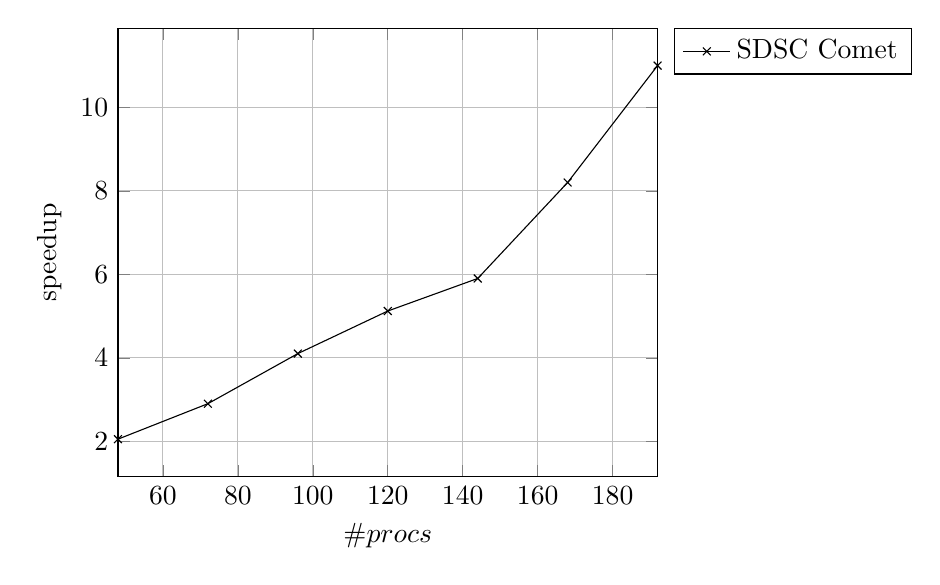
\begin{tikzpicture}
       \begin{axis}[%
            ,xlabel=$\#procs$
            ,ylabel=speedup
            ,grid=major,
            ,xmin=48,
            ,xmax=192
            ,legend style={
               cells={anchor=east},
               legend pos=outer north east,
            }]
            \addplot[color=black, mark=x] coordinates {(48,2.05) (72, 2.9) (96, 4.1) (120, 5.12) (144, 5.9) (168, 8.2) (192, 11)};
            \legend{SDSC Comet}
        \end{axis}
\end{tikzpicture}
\caption{Speedup of distributed execution. \#procs denotes the involved processes on the SDSC system Comet.}
\label{fig:speedup_laplace}
\end{figure}


\begin{figure}[H]
\centering
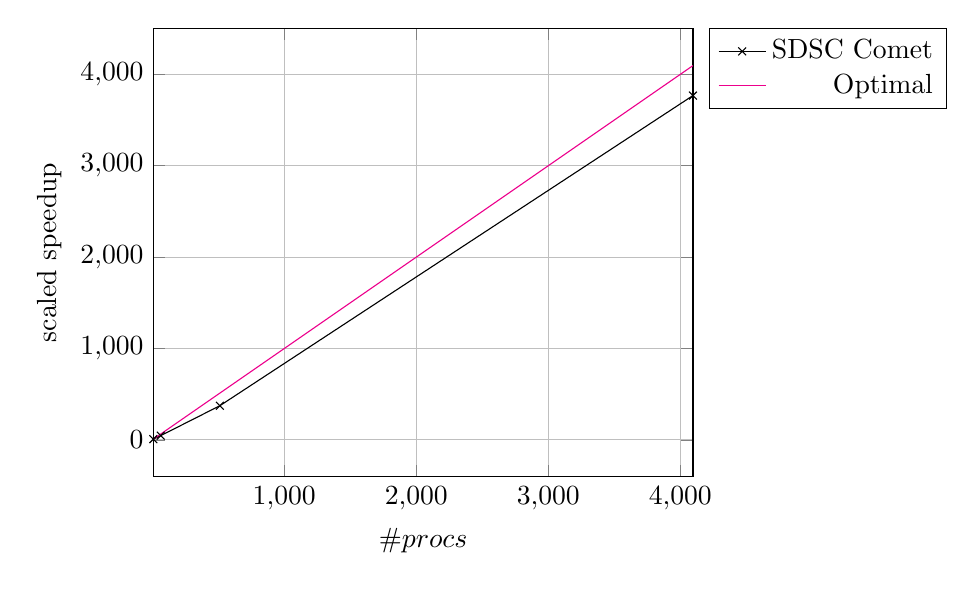
\begin{tikzpicture}
       \begin{axis}[%
            ,xlabel=$\#procs$
            ,ylabel=scaled speedup
            ,legend style={
               cells={anchor=east},
               legend pos=outer north east,
            }
            ,grid=major
            ,xmin=8,
            ,xmax=4096]
            \addplot[color=black,mark=x] coordinates {(8, 8.0) (64, 46.7) (512, 374.0) (4096, 3768.0) };
            \addplot[color=magenta] coordinates {(1,1) (4096, 4096)};
            \legend{SDSC Comet, Optimal}
        \end{axis}
\end{tikzpicture}
\caption{Scaled speedup of distributed execution. \#procs denotes the involved processes on the SDSC 
system Comet. Note the optimal scaling and achieved scaling behaviour of the test problem.}
\label{fig:scaled_speedup_laplace}
\end{figure}

%\begin{center}
%\begin{table}
%\centering
%\begin{tabular}{lrrr} 
%\toprule
%Weak scaling for benchmark problem in \ug \\
%\midrule 
%\emph{DoFs} & \emph{Total runtime [s]} & \emph{\# Processes} & \emph{\# Grid refinements} \\
%\midrule 
%27 & 1 & 1 & 0 \\
%216 & 1 & 8 & 1 \\
%1,726 & 1 & 64 & 2 \\
%13,824 & 1 & 512 & 3 \\
%110,592 & 1 & 4096 & 4 \\
%884,736 & 2 & 32768 & 5 \\
%\bottomrule
%\end{tabular}
%\caption{\textcolor{red}{Throw this out?}\sout{Runtimes of simulations of a \textbf{3d Laplace problem} on a unit cube 
%domain (different number of regular refinements) with \ug on the TACC Stampede2 HPC cluster.
%Note that each grid refinement increases the DoFs by a factor of 8. Note that the \textbf{large} queue
%on Stampede2 is not yet available to us to benchmark, thus we are restricted to process count up to 32,768.}}
%\label{fig:xsede_weak_scaling}
%\end{table}
%\end{center}

%\begin{figure}
%\centering
%\begin{tikzpicture}
%       \begin{axis}[%
%            ,xlabel=$\#procs$
%            ,ylabel=scaled speedup
%            ,legend style={
%               cells={anchor=east},
%               legend pos=outer north east,
%            }
%            ,grid=major
%            ,xmin=8,
%            ,xmax=262144
%            ,ymin=1
%            ,ymax=262144]
%            \addplot[color=black,only marks,mark=x] coordinates { (1,1) (32768, 30000) (262144, 240000)};
%            \addplot[color=magenta] coordinates {(1,1) (32768, 32678) (262144, 262144) };
%            \legend{Stampede2, Optimal}
%        \end{axis}
%\end{tikzpicture}
%\caption{Scaled speedup of distributed execution. \#procs denotes the involved processes on the TACC system Stampede2. Note the optimal scaling and achieved scaling behaviour of the test problem.}
%\label{fig:scaled_speedup_laplace2}
%\end{figure}
% }}}

% Spine model{{{
\subsection*{Subproject 1: Dendritic spine calcium simulations}
{For this subproject we ran simulations with 0 refinements (20,605 DoFs) and 1 refinement (164,840 DoFs) on Spine-Dendrite geometries that contain no ER, with simulation end time 0.02 seconds. Figure ~\ref{fig:spine_dend_strongscaling2} demonstrates the strong scaling behavior of the simulations. In particular, the geometry with 164,840 DoFs was used in running our \texttt{Baseline run} (from our previous proposal) to get a lower bound on the number of SUs. We ran with a walltime 60 minutes and the simulation consumed 40 SUs when parallelized across 512 processors. Therefore, we anticipate that each \texttt{Single Pulse run} will use at least 40 core-hours for a simulation end time of 0.02 seconds on the Expanse hpc services, and \texttt{TMS runs} will use approximately 500 SUs for an endtime of 0.25 seconds.} Our resource Table 1 is based on this preliminary run, we scaled accordingly the number of service units for the \texttt{Low-Threshold Pulse runs} which require a minimum of 1 second of simulation time.
\begin{figure}[H]
\centering
\subfigure[]{
\resizebox{0.4\textwidth}{0.4\textwidth}{%
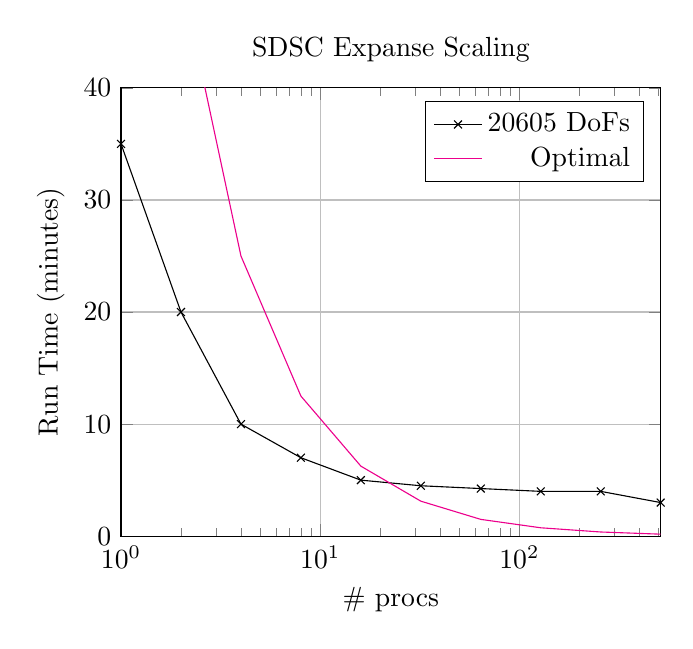
\begin{tikzpicture}
       \begin{axis}[%
       title = SDSC Expanse Scaling,
       	xmode=log,
	%ymode=log,
            ,xlabel=$\#$ procs
            ,ylabel=Run Time (minutes)
            ,grid=major,
            ,xmin=1,
            ,xmax=512,
            ,ymin=0,
            ,ymax=40,
            ,legend style={
               cells={anchor=east},
               legend pos=north east,
            }]
            \addplot[color=black,mark=x] coordinates {(1,35) (2,20) (4,10) (8,7) (16,5) (32,4.5) (64,4.25) (128,4) (256,4) (512,3)};
            \addplot[color=magenta] coordinates {(2,50) (4,25) (8,12.5) (16,6.25) (32,3.125) (64, 1.5) (128,0.75) (256,0.375) (512,0.18)};
            \legend{20605 DoFs, Optimal}
        \end{axis}
\end{tikzpicture}}}
\subfigure[]{
\resizebox{0.4\textwidth}{0.4\textwidth}{%
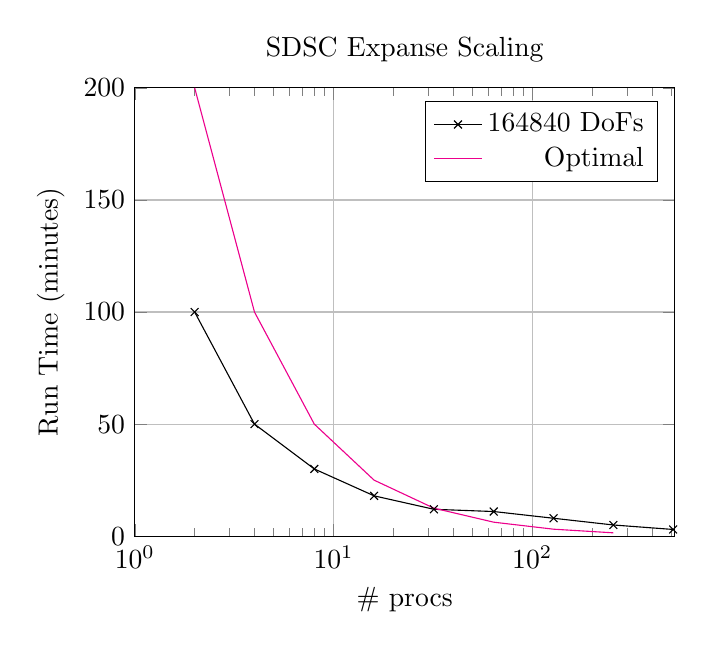
\begin{tikzpicture}
       \begin{axis}[%
       title = SDSC Expanse Scaling,
       	xmode=log,
	%ymode=log,
            ,xlabel=$\#$ procs
            ,ylabel=Run Time (minutes)
            ,grid=major,
            ,xmin=1,
            ,xmax=520,
            ,ymin=0,
            ,ymax=200,
            ,legend style={
               cells={anchor=east},
               legend pos=north east,
            }]
            %\addplot[color=blue,mark=o] coordinates {(24,59.83) (48,36.78) (96,25.72) (192,16.53) (288,18.82)};
            \addplot[color=black,mark=x] coordinates {(2, 100) (4, 50) (8,30) (16,18) (32,12) (64,11) (128,8) (256,5) (512,3)};
            \addplot[color=magenta] coordinates {(2,200) (4,100) (8,50) (16,25) (32, 12.5) (64, 6.25) (128, 3.125) (256, 1.5)};
            \legend{164840 DoFs, Optimal}
        \end{axis}
\end{tikzpicture}} }
\caption{\textit{Strong Scaling} Here we 
demonstrate the strong scaling nature of a Spine-Dendrite Calcium simulation using a spine dendrite geometry \textit{without ER}: Figure (a) 20,650 DoFs (0 refinement) and Figure (b) 164,840 DoFs (1 refinement) using the XSEDE Expanse account resources with 0.02 s end time.}
\label{fig:spine_dend_strongscaling2}
\end{figure}

%\begin{figure}[H]
%\centering
%\subfigure[]{
%\resizebox{0.4\textwidth}{0.4\textwidth}{%
%\begin{tikzpicture}
 %      \begin{axis}[%
  %     title = SU Usage 20650 DoFs,
       	%xmode=log,
	%ymode=log,
    %        ,xlabel=$\#$Processors
       %     ,ylabel=Service Units (su's)
       %     ,grid=major,
       %     ,xmin=12,
      %      ,xmax=400,
       %     ,ymin=0,
        %    ,ymax=30,
         %   ,legend style={
          %     cells={anchor=east},
           %    legend pos=north east,
      %      }]
      %      \addplot[color=black,mark=x] coordinates {(24,3) (48,3) (96,5) (192,8) (384,23)};
        %     \end{axis}
%\end{tikzpicture}} }
%\subfigure[]{
%\resizebox{0.4\textwidth}{0.4\textwidth}{%
%\begin{tikzpicture}
 %      \begin{axis}[%
  %     title = SU Usage 164840 DoFs  ,
       	%xmode=log,
	%ymode=log,
   %         ,xlabel=$\#$Processors
    %        ,ylabel=Service Units (su's)
     %       ,grid=major,
      %      ,xmin=0,
       %     ,xmax=400,
        %    ,ymin=0,
         %   ,ymax=40,
     %       ,legend style={
     %          cells={anchor=east},
     %          legend pos=north east,
     %       }]
     %       \addplot[color=black,mark=x] coordinates {(24,15) (48,18) (96,20) (192,21) (384, 29)};
      %  \end{axis}
%\end{tikzpicture}} }

%\caption{Service unit consumption, \textit{without ER}, for Figure (a) 20,650 DoFs (0 refinement) and Figure (b) 164,840 DoFs (1 refinement) using the trial XSEDE (Comet) account resources with 0.02 ms end time.}
%\label{fig:spine_dend_noERsu}
%\end{figure}

%\clearpage
%\begin{figure}[H]
%\centering
%\begin{tikzpicture}
 %      \begin{axis}[%
  %     title = SDSC Service Unit Consumption
 %           ,xlabel=$\#$Processors
 %           ,ylabel=Service Units (su's)
 %           ,grid=major,
 %           ,xmin=0,
 %           ,xmax=300,
 %           ,ymin=0,
 %           ,ymax=400,
 %           ,legend style={
 %              cells={anchor=east},
 %              legend pos=outer north east,
 %           }]
 %           \addplot[color=black,mark=x] coordinates {(24,24) (48, 29) (96, 41) (192,53) (288,90)};
 %           \addplot[color=red,mark=o] coordinates {(24,178) (48, 199) (96, 230) (192,331) (288,302)};
 %           \legend{20650 DoFs,164840 DoFs}
 %       \end{axis}
%\end{tikzpicture}
%\caption{Service Unit consumptions for Spine-Dendrite simulation runs \textit{with ER} present.}
%\label{fig:spindend_su}
%\end{figure}
\begin{figure}[H]
\centering
\resizebox{0.4\textwidth}{0.4\textwidth}{%
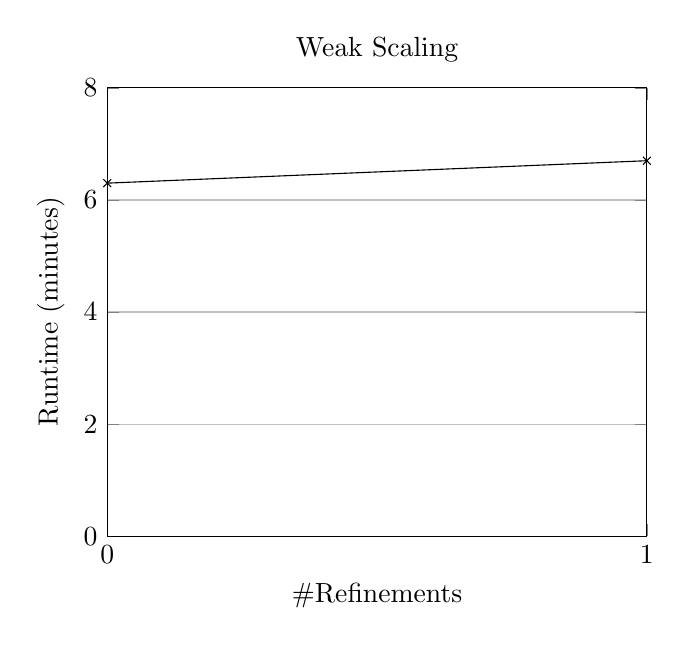
\begin{tikzpicture}
       \begin{axis}[%
       title = Weak Scaling
            ,xlabel=$\#$Refinements
            ,ylabel=Runtime (minutes)
            ,xtick={0,1,2}
            ,grid=major,
            ,xmin=0,
            ,xmax=1,
            ,ymin=0,
            ,ymax=8
            ]
            \addplot[color=black,mark=x] coordinates {(0,6.3) (1, 6.7)};
        \end{axis}
\end{tikzpicture} }
\caption{Weak Scaling for Spine-Dendrite simulation runs \textit{without ER} (using our prior allocation COMET) present with respect to Refinement level and runtime. For 0 refinement, 24 procs. were used and for 1 refinement 192 procs. were used.}
\label{fig:spindend_weakscale}
\end{figure}

% }}}

% Whole cell dynamics {{{
\subsection*{Subproject 2: Whole-cell calcium simulations}

For the whole-cell calcium model a strong and weak scaling study was conducted on
SDSC Comet, see Fig. 
\ref{fig:scaled_speedup_whole_cell} and \ref{fig:scaled_speedup_whole_cell_strong} for runtimes and Table 
\ref{tab:speedup_whole_cell} and \ref{tab:speedup_whole_cell_strong} for the associated problem sizes.

\begin{figure}[H]
\centering
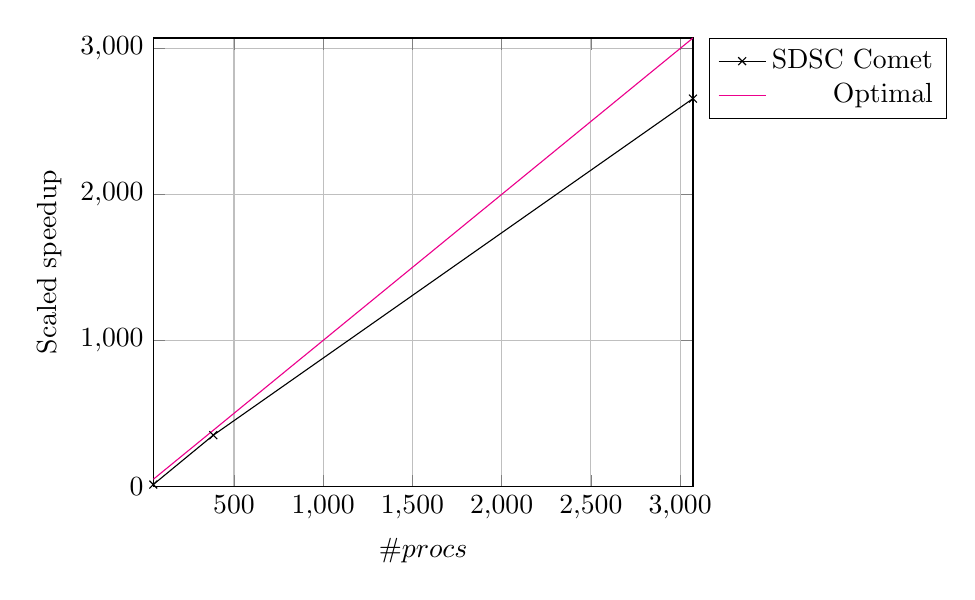
\begin{tikzpicture}
       \begin{axis}[%
            ,xlabel=$\#procs$
            ,ylabel=Scaled speedup
            ,grid=major,
            ,xmin=48,
            ,xmax=3072,
            ,ymin=0,
            ,ymax=3072,
            ,legend style={
               cells={anchor=east},
               legend pos=outer north east,
            }]
            \addplot[color=black,mark=x] coordinates {(48,12.09029345) (384, 350.144508) (3072, 2656.864865)};
            \addplot[color=magenta] coordinates {(48,48) (3072, 3072)};
            \legend{SDSC Comet, Optimal}
        \end{axis}
\end{tikzpicture}
\caption{Weak scaling result for the subproject \emph{whole-cell calcium dynamics}. 
Scaled speedup of distributed execution, where \#procs denotes the involved 
processes on SDSC Comet, shows scaling behavior for whole-cell dynamics. Problem sizes are illustrated in Table \ref{tab:speedup_whole_cell}.}
\label{fig:scaled_speedup_whole_cell}
\end{figure}

\begin{center}
\begin{table}[H]
\centering
\begin{tabular}{lrrr} 
\toprule
\emph{DoFs} & \emph{Runtime [s]} & \emph{\# Processes} & \emph{\# Refinements}\\
\midrule 
7,056 & 278 & 48 & 0 \\
56,448 & 384 & 346 & 1 \\
451,485 & 370 & 3072 & 2 \\
\bottomrule
\end{tabular}
\caption{Weak scaling result for whole cell dynamics, geometry sizes and number of involved processes on SDSC Comet.}
\label{tab:speedup_whole_cell}
\end{table}
\end{center}

\begin{figure}[H]
\centering
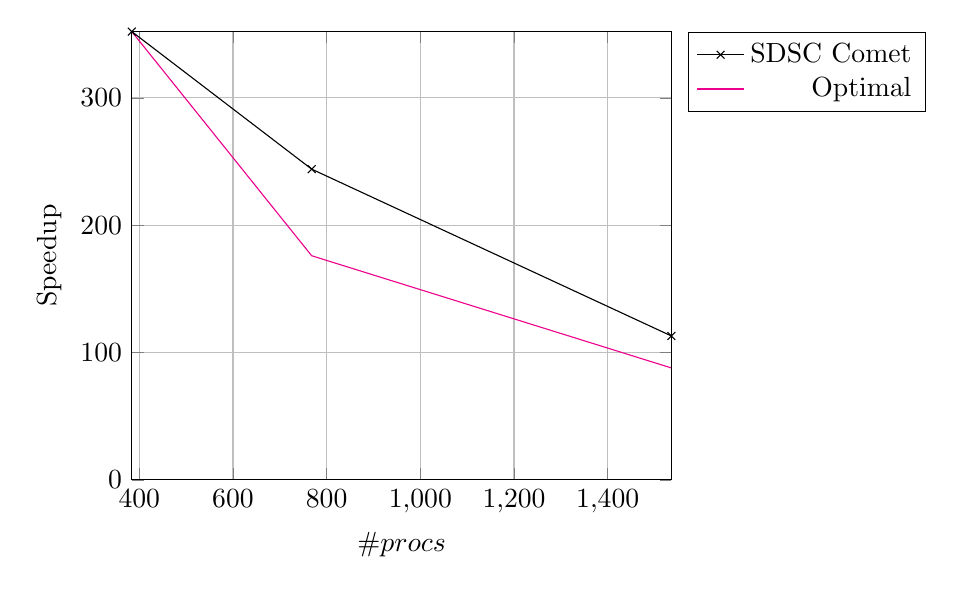
\begin{tikzpicture}
       \begin{axis}[%
            ,xlabel=$\#procs$
            ,ylabel=Speedup
            ,grid=major,
            ,xmin=384,
            ,xmax=1536,
            ,ymin=0,
            ,ymax=352,
            ,legend style={
               cells={anchor=east},
               legend pos=outer north east,
            }]
            \addplot[color=black,mark=x] coordinates {(384,352) (768, 244) (1536, 113)};
            \addplot[color=magenta] coordinates {(384,352) (768, 176) (1535, 88)};
            \legend{SDSC Comet, Optimal}
        \end{axis}
\end{tikzpicture}
\caption{Strong scaling result for the subproject whole-cell calcium dynamics. Scaled speedup of distributed execution, where \#procs denotes the involved 
processes on SDSC Comet, demonstrate scaling behavior. Problem sizes are
illustrated in Table \ref{tab:speedup_whole_cell}.}
\label{fig:scaled_speedup_whole_cell_strong}
\end{figure}

\begin{center}
\begin{table}[H]
\centering
\begin{tabular}{lrrr} 
\toprule
\emph{DoFs} & \emph{Runtime [s]} & \emph{\# Processes} & \emph{\# Nodes}\\
\midrule 
451,485 & 352 & 384 & 16 \\
451,485 & 244 & 768 & 32 \\
451,485 & 123 & 1536 & 64 \\
\bottomrule
\end{tabular}
\caption{Strong scaling results fo whole-cell dynamics, geometry sizes
and number of involved processes and nodes on SDSC Comet.}
\label{tab:speedup_whole_cell_strong}
\end{table}
\end{center}

% }}}
